\section{Question 2}
\begin{enumerate}
  \item La table~\ref{tab:val} montre différentes valeurs obtenues pour les notes de test.
    \begin{mytable}{val}{Table de différentes valeurs des notes du test.}
      \begin{tabular}{ll}
        $n$                      & \np{252}\\
Moyenne                  & \np{1.059524e+01}\\
M\'ediane                & \np{1.050000e+01}\\
\'Ecart-type             & \np{2.642711e+00}\\
\'Etendue                & \np{1.250000e+01}\\
Coefficient de variation & \np{2.494244e-01}\\
Proportion de r\'eussite & \np{3.452381e-01}\\

      \end{tabular}
    \end{mytable}
  \item Utilisons la méthode des moments
    (qui donne la même chose que celle du maximum de vraisemblance pour
    une loi normale de toute façon).
    \begin{itemize}
      \item
        Pour la loi normale, on a
        \begin{align*}
          \bar{y} & = E(Y)
                    = \mu\\
          \bar{y^2} & = E(Y^2)
                      = \var(Y) + E(Y)^2
                      = \sigma^2 + \mu^2
        \end{align*}
        ce qui donne
        \begin{align*}
          \mu & = \bar{y}\\
          \sigma^2 & = \bar{y^2} - \bar{y}^2.
        \end{align*}
      \item
        Pour la loi de Weibull, on a
        \begin{align*}
          \bar{y} & = E(Y)
                   = \sqrt[m]{\alpha}\Gamma\left(1 + \frac{1}{m}\right)\\
          \bar{y^2} & = E(Y^2)
                     = \var(Y) + E(Y)^2
                     = \alpha^{2/m}\left(\Gamma\left(1 + \frac{2}{m}\right) -
                    \Gamma^2\left(1 + \frac{1}{m}\right)\right) + \alpha^{2/m}\Gamma^2\left(1 + \frac{1}{m}\right)
                     = \alpha^{2/m}\Gamma\left(1 + \frac{2}{m}\right)
        \end{align*}
        D'où
        \begin{align*}
          \alpha & = \left(\frac{\bar{y}}{\Gamma\left(1 + \frac{1}{m}\right)}\right)^m\\
          \bar{y^2} & = \left(\frac{\bar{y}}{\Gamma\left(1 + \frac{1}{m}\right)}\right)^2\Gamma\left(1 + \frac{2}{m}\right)
        \end{align*}
        ce qui peut être résolu numériquement.
    \end{itemize}
  \item
    La figure~\ref{fig:distrib} donne quelques exemple de distribution normale et de Weibull.
    On remarque que la distribution de Weibull a $f(x; \alpha, m) = 0$ $\forall x \leq 0$
    ce qui a du sens dans ce cas car une note ne peut pas être négative alors que
    la distribution normale a $f(x) > 0$ pour $f \leq 0$ même si la valeur est très faible
    si $\mu > 0$ et que $\sigma^2$ est suffisamment petit.

    \begin{figure}
      \centering
      \begin{subfigure}[b]{0.4\textwidth}
        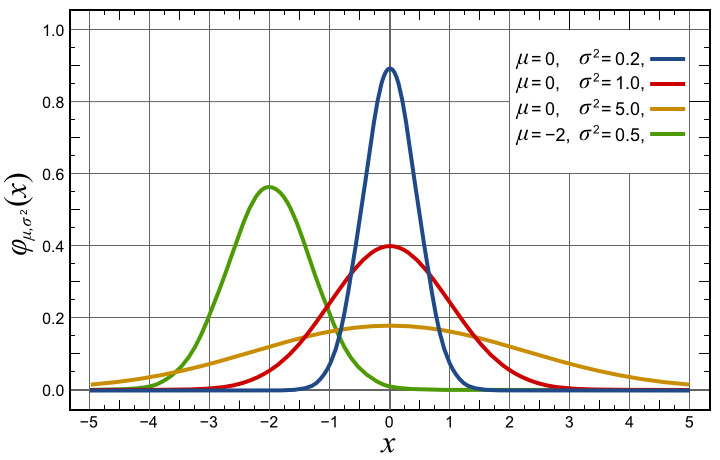
\includegraphics[width=\textwidth]{img/normal.png}
        \caption{Normal distribution}
        \label{fig:normal}
      \end{subfigure}%
      ~ %add desired spacing between images, e. g. ~, \quad, \qquad etc.
      %(or a blank line to force the subfigure onto a new line)
      \begin{subfigure}[b]{0.4\textwidth}
        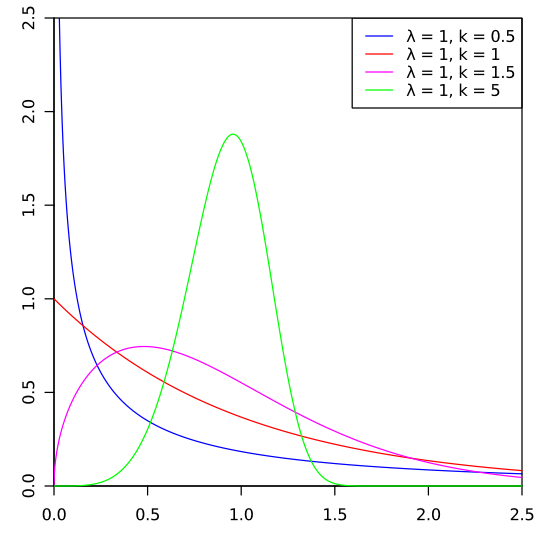
\includegraphics[width=\textwidth]{img/weibull}
        \caption{Weibull distribution}
        \label{fig:weibull}
      \end{subfigure}
      \caption{Comparison for Weibull and Normal distributions}
      \label{fig:distrib}
    \end{figure}
    De plus, la distribution normale est symétrique autour de $\mu$ alors que la distribution
    des notes d'un test n'est pas spécialement symétrique.

    À l'aide de la question précédente, on peut écrire
    \lstinline|mynormfit| (voir le listing~\ref{lst:mynormfit}) et
    \lstinline|mywblfit| (voir le listing~\ref{lst:mywblfit}).
    On peut ensuite comparer le CDF des distributions obtenues
    avec la figure~\ref{fig:cmp}.
    On remarque qu'ils sont fort semblables.

    On va donc garder la Weibull pour les raisons mentionnées plus haut.
    De toute façon, par le TCL, pour la suite,
    on pourra considérer que c'est une normale.
    \matlabplot{cmp}{Comparaisons des CDF de Weibull et de la normale avec celui des notes du test.}
  \item
    Il y a plusieurs interprétation à un étudiant moyen.
    Ça pourrait être le median ou la moyenne.
    Considérons ici que c'est la moyenne, comme elle vaut 10.6 et que la réussite est à 12,
    il ne réussira probablement pas son examen.
  \item On a calculé que $\hat{p} = \si{34.5}{\%}$.
    On sait que
    \[ \hat{p} \sim \mathcal{N}(p,\frac{p(1-p)}{n}) \]
    on a donc, en approximant $p$ au dénominateur par $\hat{p}$,
    \[ P(-z_{\alpha/2} \leq \frac{\hat{p}-p}{\sqrt{\frac{\hat{p}(1-\hat{p})}{n}}}
    \leq z_{\alpha/2}) = 1-\alpha \]
    avec $z_{\alpha/2} = 1.96$ car $\alpha = 0.05$.
    On a alors comme intervalle
    \[ \left[\hat{p}-z_{\alpha/2}\sqrt{\frac{\hat{p}(1-\hat{p})}{n}};
    \hat{p}+z_{\alpha/2}\sqrt{\frac{\hat{p}(1-\hat{p})}{n}}\right] =
    [0.287; 0.404].
    \]
  \item
    Il est hors de l'intervalle de confiance qui était un
    intervalle sûr à $\si{95}{\%}$.
    Malgrés la dualité entre intervalle de confiance et
    test d'hypothèse,
    faisons un test de l'hypothèse $H_0: p = 0.8$
    en prenant $H_1: p < 0.8$.
    Prenons $\alpha = 0.05$.
    On a à nouveau
    \[ \hat{p} \sim \mathcal{N}(p,\frac{p(1-p)}{n}) \]
    mais gardons ici $p$ au dénominateur comme il est connu
    comme on va supposer $H_0$ pour calculer $R$ tel que
    $\alpha = 0.05$.
    On remarque qu'on a, en supposans $p = p_0 = 0.8$
    \[ P(\frac{\hat{p}-p_0}{\sqrt{\frac{p_0(1-p_0)}{n}}}
    \leq -z_{\alpha}) = \alpha \]
    et donc
    \[ P(\hat{p} \leq p_0-z_{\alpha}\sqrt{\frac{p_0(1-p_0)}{n}}) = \alpha. \]
    L'ensemble $R = \{\hat{p} \in [0;1] | \hat{p} \leq p_0-z_{\alpha}\sqrt{\frac{p_0(1-p_0)}{n}}\}$
    semble donc être un candidat idéal.
    On a $p_0-z_{\alpha}\sqrt{\frac{p_0(1-p_0)}{n}} = 0.759$
    car $z_\alpha = 1.645$.
    Comme $\hat{p} = 0.345 \leq 0.759$, je me permet donc je rejetter
    $H_0$.
\end{enumerate}
